\documentclass[a4paper,norsk, 10pt]{article}
\usepackage[utf8]{inputenc}
\usepackage{verbatim}
\usepackage{listings}
\usepackage{graphicx}
\usepackage[norsk]{babel}
\usepackage{a4wide}
\usepackage{color}
\usepackage{amsmath}
\usepackage{float}
\usepackage{amssymb}
\usepackage[dvips]{epsfig}
\usepackage[toc,page]{appendix}
\usepackage[T1]{fontenc}
\usepackage{cite} % [2,3,4] --> [2--4]
\usepackage{shadow}
\usepackage{hyperref}
\usepackage{titling}
\usepackage{marvosym }
\usepackage{subcaption}
\usepackage[noabbrev]{cleveref}
\usepackage{cite}
\newcommand{\pd}[2]{\frac{\partial #1}{\partial #2}}
\setlength{\droptitle}{-10em}   % This is your set screw

\setcounter{tocdepth}{2}

\lstset{language=c++}
\lstset{alsolanguage=[90]Fortran}
\lstset{alsolanguage=Python}
\lstset{basicstyle=\small}
\lstset{backgroundcolor=\color{white}}
\lstset{frame=single}
\lstset{stringstyle=\ttfamily}
\lstset{keywordstyle=\color{red}\bfseries}
\lstset{commentstyle=\itshape\color{blue}}
\lstset{showspaces=false}
\lstset{showstringspaces=false}
\lstset{showtabs=false}
\lstset{breaklines}
\title{FYS2160 Oblig 3}
\author{Daniel Heinesen, daniehei}
\begin{document}
\maketitle

\section{Project 3}
We have Helmholtz free energy for the van der Waals gas:

\begin{equation}
F_{wdW} = -NkT\left[\ln\left(\frac{n_Q(V-Nb)}{N}\right) + 1 \right] - \frac{aN^2}{V}
\label{eq:freeEnergy}
\end{equation}

with $n_Q(T) = (2\pi mkT/h^2)^{3/2}$

\subsection{a)}
We can find the pressure from this by the thermodynamic identity

\begin{equation}
P(N,V,T) = -\left(\pd{F}{V}\right)_{T,N}
\label{eq:formPressure}
\end{equation}

If we calculate the pressure for \eqref{eq:freeEnergy} we find

\begin{equation}
P(N,V,T) = -\left(-NkT\frac{N}{n_Q(V-Nb)}\cdot\frac{n_Q}{N} + \frac{aN^2}{V^2}\right) = \frac{NkT}{V-Nb} - \frac{aN^2}{V^2}
\label{eq:waalsP}
\end{equation}

\subsection{b)}

We now introduce
\begin{equation}
P_c = \frac{a}{27b^2}, \qquad V_c = 3Nb, \qquad kT_c = \frac{8a}{27b}
\end{equation}

and 

\begin{equation}
\hat{P} = P/P_c, \qquad \hat{V} = V/V_c \qquad \hat{T} = T/T_c
\end{equation}

with the density

\begin{equation}
\hat{\rho} = 1/\hat{V} =  \rho/\rho_c,\qquad \rho_c = \frac{1}{3b}
\label{eq:dimless_rho}
\end{equation}

We can thus write the pressure of the van der Waals gas \eqref{eq:waalsP} dimensionless:

\begin{equation*}
P = \hat{P}P_c =  \frac{Nk\hat{T}T_c}{\hat{V}V_c-Nb} - \frac{aN^2}{\hat{V}^2 V_c^2}
\label{eq:scaling}
\end{equation*}

\begin{equation*}
\hat{P}\frac{a}{27b^2} = \frac{Nk\hat{T}\frac{8a}{27bk}}{\hat{V}3Nb-Nb} - \frac{aN^2}{\hat{V}^2 9N^2b^2}
\end{equation*}

\begin{equation}
\hat{P} = \frac{27b^2}{a}\left(\frac{a}{27b^2}\frac{\hat{8T}}{3\hat{V} - 1} - \frac{a}{27b^2}\frac{3}{\hat{V}^2}\right) = \frac{\hat{8T}}{3\hat{V} - 1} - \frac{3}{\hat{V}^2}
\label{eq:dimlessPress_vol}
\end{equation}

\subsection{c)}

If we plot the pressure \eqref{eq:dimlessPress_vol} we get

\begin{figure}[H]
\centering
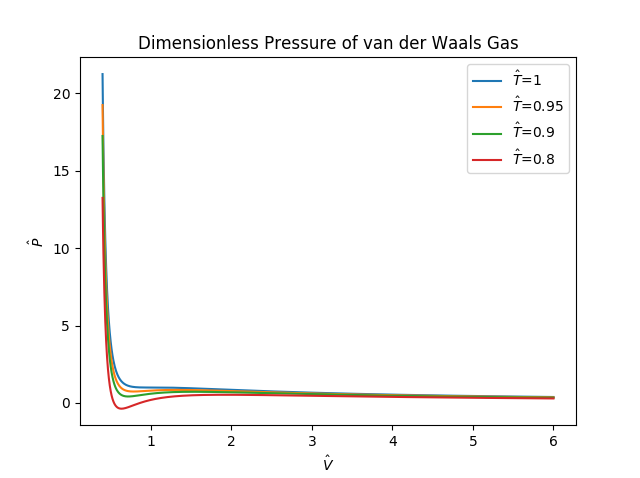
\includegraphics[scale=0.5]{p3c.png}
\caption{We see that around $\hat{V} = 1$ we pressure as a function of $\hat{V}$ is non-injective, this means that we are unable to find an inverse $\hat{V}(\hat{P})$.}
\end{figure}

\subsection{d)}
We saw in \eqref{eq:dimless_rho} that we can write the density as $\hat{\rho} = 1/\hat{V}$. Using this in \eqref{eq:dimlessPress_vol} we get

\begin{equation}
\hat{P} = \frac{\hat{8T}}{3/\hat{\rho} - 1} - \frac{3}{1/\hat{\rho}^2} = \frac{8\hat{\rho}\hat{T}}{3-\hat{\rho}} - 3\hat{\rho}^2
\label{eq:dimlessPress_dens}
\end{equation}

\subsection{e)}
We can so plot the pressure against density:

\begin{figure}[H]
\centering
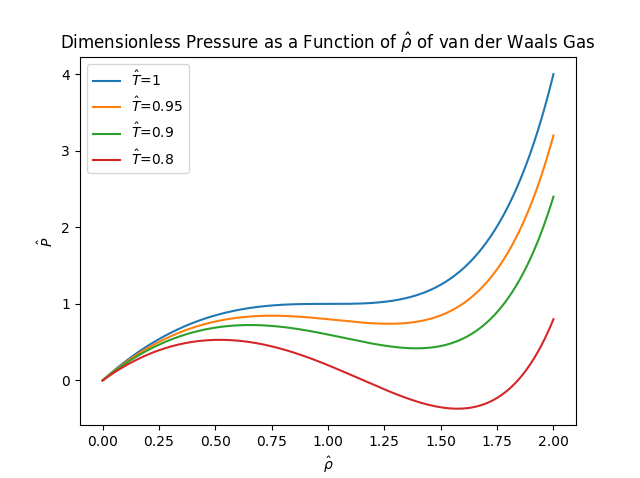
\includegraphics[scale=0.5]{p3e.png}
\caption{The pressure of the van der Waals gas as a function of $\hat{\rho}$}
\label{fig:press_rho}
\end{figure}

\subsection{f)}
As seen in fig. \ref{fig:press_rho}, for $\hat{T} \geq 1$ does pressure become an injective function of the density. This means that we can find an inverse $\hat{\rho}(\hat{V})$. This will be unique. This means that for $\hat{T} < 1$ there will be no such unique function.\\

 (\textbf{Dette virker bare rart, sjekk dette før du leverer!!!!!})

\subsection{g)}

We want to see where the isothermal compressibility is negative:

\begin{equation}
\kappa = \frac{1}{\rho}\left(\pd{\rho}{P}\right) < 0
\end{equation}

We see that this happens when $\partial \rho/\partial P < 0$, which is the same as saying that $\partial P/\partial \rho < 0$. We can see from figure \ref{fig:press_rho} that this happens for every temperature except $\hat{T} = 1$ around $0.5 \leq \hat{\rho} \leq 1.55$ (more or less). We can also compute this numerically

\begin{figure}[H]
\centering
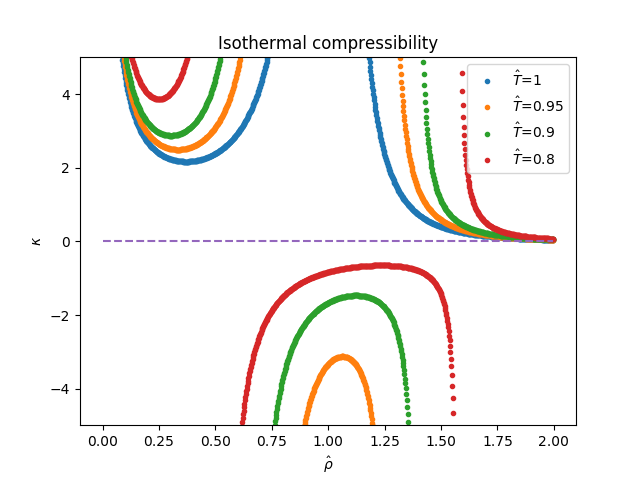
\includegraphics[scale=0.5]{isoComp.png}
\caption{The isothermal compressibility as function of $\hat{\rho}$.}
\label{fig:isoComp}
\end{figure}

We can see that our approximation of the range of $\hat{\rho}$ was pretty good for $\hat{T} = 0.8$, and as the temperature raises this interval becomes narrower, until for $\hat{T} = 1$ $\kappa$ is positive for all $\hat{rho}$.


\subsection{h)}
We are going to look at the PV isotherms of $N_2$. To do this use \eqref{eq:dimlessPress_vol} and \eqref{eq:scaling} to find

\begin{equation}
P = P_c\left[\frac{\hat{8T/T_c}}{3\hat{V}/V_c - 1} - \frac{3V_c^2}{\hat{V}^2}\right]
\end{equation}

Where

\begin{equation}
P_c = 33.6 \text{ atm}, \qquad V_c = 0.089 \text{ l/mol}, \qquad T_c = 126 \text{ K}
\end{equation}

If we plot this for $T = 77,100,110,115,120,125$ K we get

\begin{figure}[H]
\centering
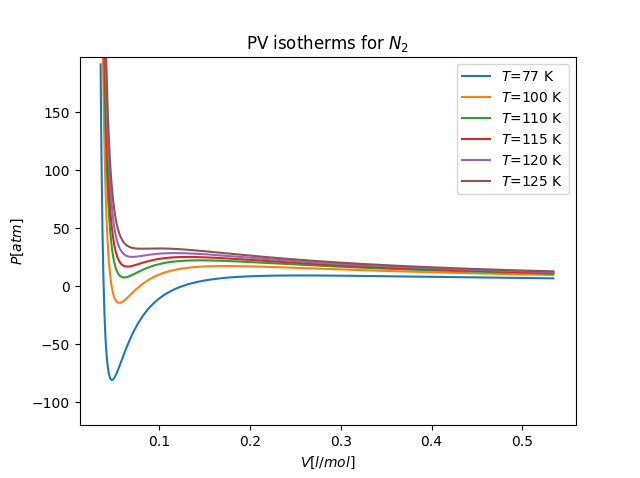
\includegraphics[scale=0.5]{isoTherm.png}
\caption{The PV isotherms for $N_2$.}
\label{fig:isoTherm}
\end{figure}

\subsection{i)}


\subsection{j)}

\section{Project 4}
\subsection{a)}
We start with expanding $dS$ and $dV$

\begin{equation}
ds = \left(\pd{S}{T}\right)_V dT + \left(\pd{S}{V}\right)_T dV
\label{eq:ds}
\end{equation}
\begin{equation}
dV = \left(\pd{V}{T}\right)_P dT + \left(\pd{V}{P}\right)_T dP
\label{eq:dV}
\end{equation}

If we insert the expression for $dV$ into that of $dS$, we get

\begin{equation}
dS = \left(\pd{S}{T}\right)_V dT + \left(\pd{S}{V}\right)_T\left[\left(\pd{V}{T}\right)_P dT + \left(\pd{V}{P}\right)_T dP\right]
\end{equation}

If we sort the expression we get:

\begin{equation}
dS = \left[\left(\pd{S}{T}\right)_V + \left(\pd{S}{V}\right)_T\left(\pd{V}{T}\right)_P\right]dT + \left(\pd{S}{V}\right)_T\left(\pd{V}{P}\right)_T dP
\end{equation}

We are looking at the heating with constant pressure, so $dP = 0$ and

\begin{equation}
dS = \left[\left(\pd{S}{T}\right)_V + \left(\pd{S}{V}\right)_T\left(\pd{V}{T}\right)_P\right]dT \Leftrightarrow \left(\pd{S}{T}\right)_P = \left(\pd{S}{T}\right)_V + \left(\pd{S}{V}\right)_T\left(\pd{V}{T}\right)_P
\end{equation}

We can no use the identities for the heat capacities:

\begin{equation}
C_V = T\left(\pd{S}{T}\right)_V, \qquad C_P = T\left(\pd{S}{T}\right)_P
\label{eq:heatCap}
\end{equation}

and

\begin{equation}
\alpha = \frac{1}{V}\left(\pd{V}{T}\right)_P
\label{eq:alpha}
\end{equation}

Which gives us the relation

\begin{equation}
\frac{C_V}{T} = \frac{C_P}{T} + V\alpha \left(\pd{S}{V}\right)_T
\label{eq:almost}
\end{equation}

We now need an expression for the last partial differentiation. We start with a constant volume $dV = 0$, which gives from \eqref{eq:dV}

\begin{equation}
0 = \left(\pd{V}{T}\right)_P dT + \left(\pd{V}{P}\right)_T dP
\end{equation}
\begin{equation}
\Rightarrow \left(\pd{P}{T}\right)_V = - \frac{\left(\pd{V}{T}\right)_P}{\left(\pd{V}{P}\right)_T}
\end{equation}

we now use that 

\begin{equation}
\beta_T = -\frac{1}{V}\left(\pd{V}{P}\right)_T
\end{equation}

and get that

\begin{equation}
\Rightarrow \left(\pd{P}{T}\right)_V = \frac{\alpha}{\beta_T}
\end{equation}

Inserting this into \eqref{eq:almost} we get the relation for the heat capacities:

\begin{equation}
C_V = C_P + VT\frac{\alpha^2}{\beta_T}
\end{equation}

\subsection{b)}

From eq. \eqref{eq:heatCap} we get that

\begin{equation}
\frac{C_P}{C_V} = \frac{\left(\pd{S}{T}\right)_P}{\left(\pd{S}{T}\right)_V}
\label{eq:cp/cv}
\end{equation}

We now need to look at these expressions. We start with $\left(\pd{S}{T}\right)_P$. We know from this that $dP = 0$. Since the expression involves $S$ and $T$ we are going to look at $dP(S,T) = 0$

\begin{equation}
dP = 0 = \left(\pd{P}{T}\right)_S dT + \left(\pd{P}{S}\right)_T dS
\end{equation}
From this we get

\begin{equation}
\left(\pd{S}{T}\right)_P = -\frac{\left(\pd{P}{T}\right)_S}{\left(\pd{P}{S}\right)_T}
\end{equation}

We use the same logic with $\left(\pd{S}{T}\right)_V$:

\begin{equation}
dV(S,T) = 0 = \left(\pd{V}{T}\right)_S dT + \left(\pd{V}{S}\right)_T dS
\end{equation}
\begin{equation}
\Rightarrow\left(\pd{S}{T}\right)_V = -\frac{\left(\pd{V}{T}\right)_S}{\left(\pd{V}{S}\right)_T}
\end{equation}

We can now insert this into \eqref{eq:cp/cv}

\begin{equation}
\frac{C_P}{C_V} = \frac{\left(\pd{P}{T}\right)_S}{\left(\pd{V}{T}\right)_S}\frac{\left(\pd{V}{S}\right)_T}{\left(\pd{P}{S}\right)_T} =
\left(\pd{P}{V}\right)_S \left(\pd{V}{P}\right)_T
\end{equation}

We can then use that

\begin{equation}
\beta_S = -\frac{1}{V}\left(\pd{V}{P}\right)_S, \qquad \beta_T = -\frac{1}{V}\left(\pd{V}{P}\right)_T
\end{equation}

And we then get

\begin{equation}
\frac{C_P}{C_V} = \left(\pd{P}{V}\right)_S \left(\pd{V}{P}\right)_T = \frac{\beta_T}{\beta_S}
\end{equation}

\subsection{c)}
We start with the first law for pressure-volume work

\begin{equation}
dU = dQ - dW = dQ - PdV
\label{eq:firstLaw}
\end{equation}

We then, as the exercise hinted, expand $dH$. We do this for $H(T,P)$

\begin{equation}
dH = \left(\pd{H}{T}\right)_P dT + \left(\pd{H}{P}\right)_T dP
\end{equation}

But in this system $dP = 0$, so this reduces to

\begin{equation}
dH = \left(\pd{H}{T}\right)_P dT
\end{equation}

We also know that for this pressure-volume system the change enthalpy is given as

\begin{equation}
dH = dU + PdV
\end{equation}

Inserting this for $dU$ in \eqref{eq:firstLaw} we get

\begin{equation}
dQ = \left(\pd{H}{T}\right)_P dT
\end{equation}

and since we have constant pressure, we get

\begin{equation}
\left(\pd{Q}{T}\right)_P = C_P = \left(\pd{H}{T}\right)_P
\end{equation}


\end{document}

